\chapter{Testing the ArduPilot Framework}

    \section{Setup of the Drone}
        \subsection{Configuring the Raspberry Pi}
            This link \cite{emlid_rpi_config} explain how to configure the Raspberry Pi. The \textit{Upgrading} and \textit{Expanding rootfs} were not used. It recommended to not follow them if not needed.
            
            \subsubsection{Installing the Emlid image on a Raspberry Pi}
                The following commands is to check if the downloaded file is not corrupted.

                \begin{enumerate}
                    \item Download Raspbian image and the md5 file from here \cite{emlid_rpi_config} in the same folder.
                    \item open a terminal and cd to the folder (e.g. Downloads)
                    \item Decompress the raspbian image with
                    
                    \begin{minted}{bash}
# <numbers> is 20190227 at the time of redaction of this report
unxz emlid-raspbian-<numbers>.img.xz -kv
# Note: -kv (or -k -v or --keep --verbose) means keep original compressed file, v is verbose to show output in terminal.
                    \end{minted}
                
                    \item Check if the image is intact with

                    \begin{minted}{bash}
md5sum emlid-raspbian-<numbers>.img | md5sum --check
# It should return
emlid-raspbian-<numbers>.img: OK
                    \end{minted}
                
                    \item follow the section "Writing image to SD card" of the Emlid tutorial
                    \item Burn the image on a SD card.
                    \item Insert the sd card in the Raspberry Pi.
                    \item Connect a monitor and a keyboard to the Raspberry Pi. Note that even if you use an azerty keyboard, it the keys are interpreted as if it was qwerty.
                    \item Power the Raspberry Pi.
                \end{enumerate}
                You should see on the screen the Raspberry Pi booting.
                
            \subsubsection{Configuring the Raspberry Pi Wifi}
                
                \begin{enumerate}
                    \item Enter username \texttt{pi} and password \texttt{rapsberry}.
                    \item Type \texttt{sudo nano /boot/wpa\_supplicant.conf}.
                    \item Add the following line to the file. The router has different wifi band. Choose either \texttt{NETGEAR03}, \texttt{NETGEAR03-5G-1}, \texttt{NETGEAR03-5G-2} to choose which wifi band use. \texttt{NETGEAR03-5G-1} is used here. The password is written on the router.
                    
                    \begin{minted}{bash}
network={
  ssid="NETGEAR03-5G-1"
  psk="littlecoconut746"
  key_mgmt=WPA-PSK
}
                    \end{minted}
                \end{enumerate}

            \subsubsection{Configuring the Raspberry Pi Hostname}
                \begin{enumerate}
                    \item Log in to the raspberry pie
                    \item \texttt{sudo nano /etc/hostname}
                    \item Change \texttt{navio} to \texttt{navio<xx>} \texttt{<xx>} being the index.
                    \item \texttt{sudo nano /etc/hosts}
                    \item Change \texttt{navio} to \texttt{navio<xx>}.
                    \item Shutdown the Raspberry Pi with \texttt{sudo shutdown -h now}.
                    \item Whenever you want to restart the raspberry pie again after shutting it down, just unplug and plug the power cable.
                \end{enumerate}
                
        \subsection{Configuring the Router}
            \subsubsection{Connecting to the router}
                \begin{enumerate}
                    \item Power the Router
                    \item Wait for the Wifi LED to lit up.
                    \item Deconnect from all networks you are connected to. It can cause problems to access the configuration of the router.
                    \item Connect to the Wifi network \texttt{NETGEAR03} with the password \texttt{littlecoconut746}.
                    \item Go to the router configuration page \url{http://www.routerlogin.net}.
                    \item Enter the username \texttt{admin} and the password \texttt{password}.
                \end{enumerate}
                
                If you ever change the password and lost it, it can be recovered with this \ref{fig:r8000p_settings}
                
                \begin{figure}[!ht]
                    \centering
                    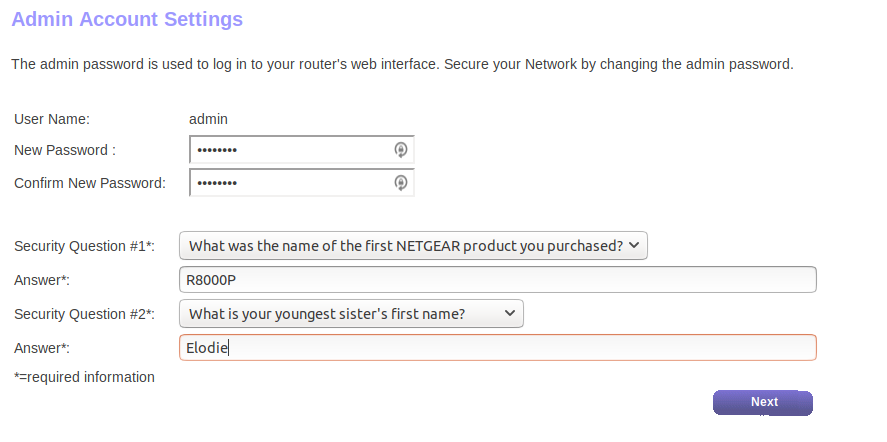
\includegraphics[width=.5\linewidth]{r8000p_settings.png}
                    \caption{Recovery Answers}
                    \label{fig:r8000p_settings}
                \end{figure}
                
                

            \subsubsection{Configuring internet}
                You can configure a connection to the internet in the WiFi network by connecting the router via an Ethernet cable.
                
            \subsubsection{Reserve fixed IP address}
                Once this is done, you reserve an LAN IP address for the Raspberry Pi and the computer using \href{https://kb.netgear.com/24091/How-do-I-reserve-a-LAN-IP-address-on-my-Nighthawk-router}{this method}.
                \begin{enumerate}
                    \item Assure that the device you want to reserve an IP address is connected to the wifi. For the Raspberry Pi, doing the preceding steps, power it up and wait a minute should be enough.
                    \item Assure that your computer is connected to the Nighthawk router with wifi. And do not connect to other network, it can cause problems (e.g. not being able to connect to http://www.routerlogin.net).
                    \item Connect to \url{http://www.routerlogin.net} in a browser.
                    \item Enter username \texttt{admin} and password \texttt{password}.
                    \item Select \emph{ADVANCED > Setup > LAN Setup}.
                    \item In the Address Reservation section of the page, click the \emph{Add} button.
                    \item You should see in the \emph{Address Reservation} the list of devices without reserved IP address.
                    \item Enter the \emph{IP Address} you want for the device. It must be between \texttt{192.168.1.2} and \texttt{192.168.1.254}. I use \texttt{192.168.1.100} for my computer and \texttt{192.168.1.1<xx>} for the \texttt{navio<xx>}.
                    \item Enter the \emph{MAC Address}, you can copy paste the MAC address from the list \emph{Address Reservation}.
                    \item Enter the \emph{Device Name}, I choose to name my computer \emph{jonathan} and the Raspberry Pi \texttt{navio<xx>}.
                    \item Click the \emph{Add} button then the \emph{Apply} button.
                \end{enumerate}
        
        \subsection{Configuring SSH connections}       
                Now, we can ssh the Raspberry Pi using on the computer
            \subsubsection{Connect via SSH}
            
                \begin{minted}{bash}
    # ssh pi@192.168.1.1<xx> to connect to the navio<xx> for example
    ssh pi@192.168.1.101 # For navio01
    #or
    ssh pi@navio01.local # For navio01
    
                \end{minted}
                
                \begin{enumerate}
                    \item If it ask you \emph{Are you sure you want to continue connecting} enter \emph{yes}.
                    \item Enter password \texttt{raspberry}.
                    \item You are normally connected to \texttt{pi@navio}.
                    \item You can enter \texttt{Ctrl+D} to logout of the Raspberry Pi.
                \end{enumerate}
                
            \subsubsection{Create an SSH key}
                To avoid writing the Raspberry Pi password every time I want to connect via ssh, I used \href{https://www.ssh.com/ssh/copy-id}{this tutorial} with some alterations. I created an ssh key on my computer and shared it to the Raspberry Pi to identify my computer automaticaly.
                
                \begin{enumerate}
                    \item open a terminal and type cd .ssh and ls. If the output is just $known_hosts$, it means you don't have keys yet.
                    \item On your computer, enter in the terminal \texttt{ssh-keygen -t rsa}.
                    \item Press enter 3 times, once to choose the default path to save the key and the last two not to use a password on the ssh key.
                    \item Enter this command
                \end{enumerate}
                
            \subsubsection{Saving your SSH key on the Raspberry Pi}
                
                \begin{minted}{bash}
ssh-copy-id pi@192.168.1.1<xx>
# or this if you have a custom ssh key
ssh-copy-id /path/to/ssh/key/file.pub pi@192.168.1.1<xx>
# You can now test, if it has worked with
ssh pi@192.168.1.1<xx> # For navio<xx>
# You are now connected to the navio without having to type a password.
                \end{minted}
    
        \subsection{Setting Ardupilot}
            Follow \href{https://docs.emlid.com/navio2/common/ardupilot/installation-and-running/}{this page} of the Emlid documentation.
                
            \begin{enumerate}
                \item \texttt{sudo emlidtool ardupilot}
                \item Select vehicle \texttt{copter}, version \texttt{3.6}, frame \texttt{arducopter}, \texttt{enable} on boot, \texttt{stop}, \texttt{Apply} and \texttt{Quit}.
                \item \texttt{sudo nano /etc/default/arducopter}
          
            
                \begin{minted}{bash}
    # Change this line
    TELEM1="-A udp:127.0.0.1:14550"
    # by this line
    TELEM1="-A udp:192.168.1.100:140<xx>"
    # You change the IP address by the one of your computer
    # Save the change
                \end{minted}
                                
           
                \item \texttt{sudo systemctl daemon-reload}
                \item \texttt{sudo emlidtool ardupilot}
                \item Select vehicle \texttt{copter}, version \texttt{3.6}, frame \texttt{arducopter}, \texttt{enable} on boot, \texttt{start}, \texttt{Apply} and \texttt{Quit}.
                \item Logout with \texttt{Ctrl+D}
                \item (outdated) You are now in the terminal of your computer. Launch now MAVPROXY. This would be automatically instulled if you follow the simulation section of ardupilot. We will use QGroundControl and MAVROS.
            \end{enumerate}
            
        \subsection{QGroundControl}
            \subsubsection{Installation}
                Install QGroundStation, follow this explanation \cite{qgc_install}.
                
                
            You will now setup QGroundControl to monitor the drones. More details can be find here \cite{qgc_setup}.{ \color{red}HAS TO BE EDITED.}
            
            \subsubsection{Telemetry}
                \begin{enumerate}
                    \item Click on the Q at the top left
                    \item Click on Comm links
                    \item Click on Add button
                    \item Fill UDP for type, navio<xx> for name, 140<xx> for Listening Port.
                    \item Click on OK
                    \item Click Connect, the screen should change to the summary page if it is successful.
                \end{enumerate}
            
            \subsubsection{Airframe}
                \begin{enumerate}
                    \item Set \texttt{Quad} as \texttt{Frame Class}.
                    \item Set \texttt{X} as \texttt{Frame Type}.
                \end{enumerate}
                
            \subsubsection{Radio}
                \begin{enumerate}
                    \item power the radio
                    \item Set \texttt{PPM} output mode for the receiver (see Section ADD REF). You should not need to modify the output mode except if you want to test individual motor.
                    \item Follow the instructions of the documentation Radio Setup.
                \end{enumerate}
                
            \subsubsection{Sensors}
                \begin{enumerate}
                    \item Calibrate Accelerometer with \texttt{None} as \texttt{Autopilot Orientation}.
                    \item Calibrate Compass, I use the two compass as they were both in the green.
                    \item Calibrate Level Horizon  with \texttt{ROTATION\_NONE} as \texttt{Autopilot Orientation}.
                    \item Calibrate Pressure.
                \end{enumerate}
                I did not use the CompassMot calibration. It may improve the drone performance. the battery current monitor would have to be configured.
                
            \subsubsection{Flight Modes}
                There is a lot of different flight for Ardupilot \href{http://ardupilot.org/copter/docs/flight-modes.html}{this}.
                \begin{enumerate}
                    \item Set \texttt{Channel 5} for the \texttt{Flight mode channel}.
                    \item Set \texttt{Alt. Hold} as \texttt{Flight Mode 1} and \texttt{Land} for the other.
                \end{enumerate}
                If something happens, you just have to turn the knob \texttt{VRA} and lower the throttle to land the drone.
                There may be a way to stop the motors directly.
                
                You can directly see which flight mode is selected in the interface for different position of the knob.
                
            \subsubsection{Power}
                You can setup the voltage and current reading in the Power windows.
                I did not explored how to set it up. Put it on disabled.
                
            \subsubsection{Safety}
                As GPS is not use on this project. All the safety setup that use GPS has to be modified.
                \begin{enumerate}
                    \item Replace \texttt{RTL} that use GPS by \texttt{Land}.
                    \item Select every arming check except \texttt{GPS Lock} and \texttt{GPS Configuration}.
                \end{enumerate}
            
    \section{Flying with RC only}
        \subsection{Checklist}
            {\color{orange} to complete} ArduPilot propose a Pre-Flight Checklist \cite{ardupilot_checklist}.
            \begin{itemize}
                \item The battery is charged.
                \item Nothing hinders the rotation of the propellers.
                \item 
            \end{itemize}
            
        \subsection{Take off process}
            \begin{enumerate}
                \item Plug the battery to the drone.
                \item Place the drone on a flat surface.
                \item Wait the for the LED to flash red and blue and then it single flash yellow. If it double flash yellow the pre-arm checks failed. More on LED meaning \href{http://ardupilot.org/copter/docs/common-leds-pixhawk.html}{here}.
                \item Power on the transmitter. The LED should flash blue.
                \item Select the flight mode on the transmitter you want to use with the knob \texttt{VRA}.
                \item Arm the drone by placing the throttle stick to the bottom right for 2 seconds. When the LED is solid blue release the throttle stick. The motor will start to spin.
                \item You can now fly the drone.
            \end{enumerate}
        
        \subsection{Landing process}
            \begin{enumerate}
                \item Place the drone where it can land straight down.
                \item Lower the throttle stick to the minimum.
                \item Select the land mode with the knob \texttt{VRA}.
            \end{enumerate}